\documentclass{gajewski}

\bibliographystyle{IEEEtran}

%%%%%%%%%%%%%%%%%
% Document variables
%%%%%%%%%%%%%%%%%
\docDate{ \today }
\docID{Present Decoder}
\docRevision{0.2}
\docStatus{Draft}
\docTitle{\mbox{Present Decoder}} 
\authorName{\mbox{Krzysztof Gajewski} \\ and opencores.org}
\authorURL{www.opencores.org}
\authorAddress{\mbox{}}
\authorEmail{gajos@opencores.org}

\revisionList{ 
0.1 & all & 2014/05/25 & First draft & K. Gajewski \\
0.2 & all & 2014/09/16 & Some small corrections with the text, typos, etc. & K. Gajewski \\
}

\begin{document}

\maketitle

\newpage

\revisionTable

\newpage

\tableofcontents
\newpage

\section{Introduction}

Present is "ultra-lightweight" block cipher developed by A. Bogdanov et al. and proposed in 2007 \cite{PRESENT}. It uses 64 bit data block and 80 bit or 128 bit key.
This cipher consists of 32 rounds, during which: 
\begin{itemize}
    \item round key is added to plaintext
    \item plaintext goes through sBoxes (substitution boxes)
    \item plaintext after sBoxes goes through pLayer (permutation layer)
    \item round key is updated
\end{itemize}
After that, ciphertext feeds out the output. Briefly algorithm was shown in Fig. \ref{pAlgorithm}.
\begin{figure}[!ht]%
    \begin{center}
    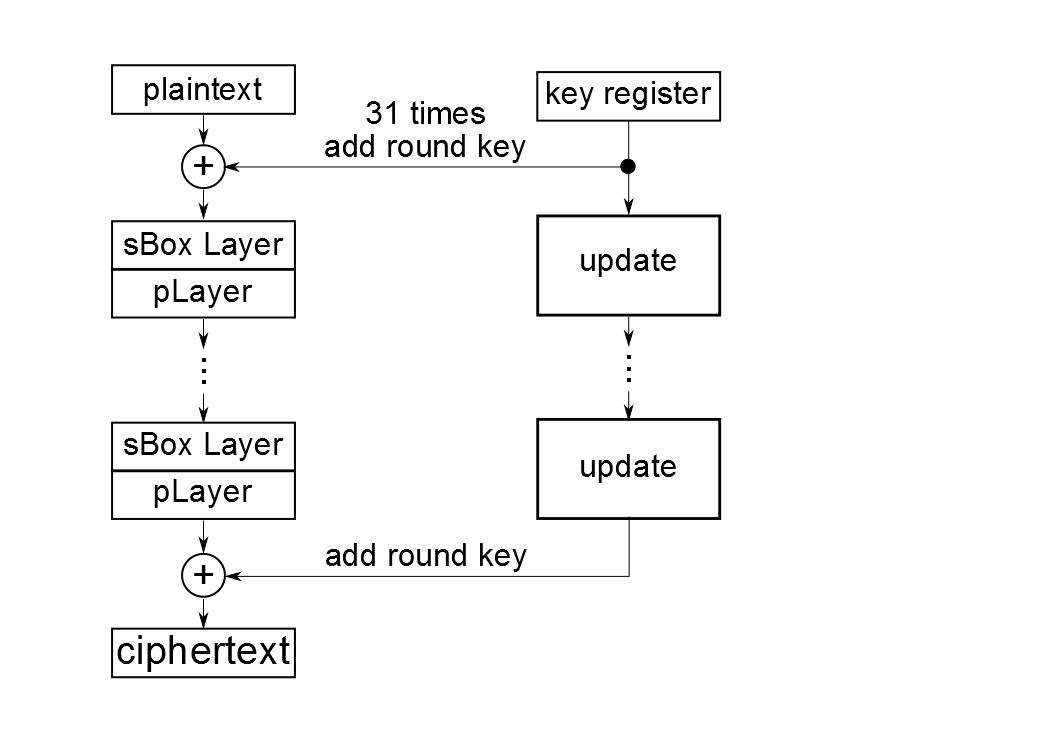
\includegraphics[width=0.66\textwidth]{img/presentAlgorithm.png}
    \caption{%
        Briefly block scheme of the PRESENT block cipher
     }%
    \label{pAlgorithm}
    \end{center}
 \end{figure}
In subprojects \texttt{Pure} and \texttt{PureTesting} Present encoder components was presented. In this subproject Present decoder was presented. Decoding key is firstly generated, basing on the key used for data coding. Next, input data are decoded (taking into account "inverse" direction to the presented in Fig. \ref{pAlgorithm}), and at last feeds the output. This core works with 80 bit key. Target was Xilinx\textsuperscript{\textregistered} Spartan 3E XC3S500E \cite{Spartan} on Spartan 3E  Starter Board \cite{Digilent} made by Digilent\textsuperscript{\textregistered}.

\newpage 

\section{Interface}

Top level component of the Present decoder was shown in Fig. \ref{pfdec}. All inputs and outputs are synchronous except \texttt{reset} signal and sampled at rising edge of the clock. Type for all signals is \texttt{STD\_LOGIC} or \texttt{STD\_LOGIC\_VECTOR}.
\begin{figure}[!ht]%
    \begin{center}
    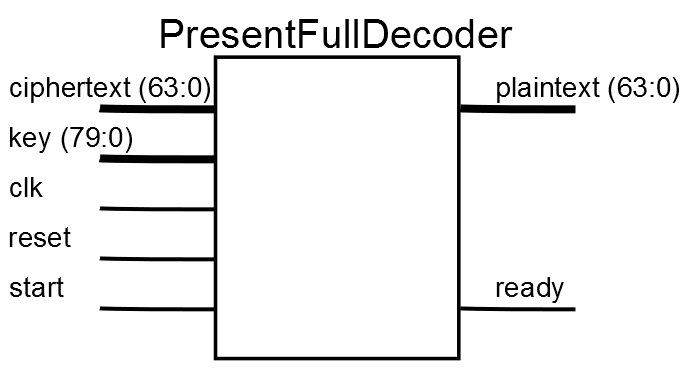
\includegraphics[width=0.5\textwidth]{img/PresentFullDecoder.png}
    \caption{%
        Top level component of the Present decoder
     }%
    \label{pfdec}
    \end{center}
 \end{figure}

\begin{tabularx}{\textwidth}{|p{30mm}|p{11mm}|p{11mm}|X|}
  \hline \bf{Signal name} & \bf{Width} & \bf{In/Out} & \bf{Description}\\ 
  \hline \texttt{ciphertext}	& 64  &  in  & input data which have to be decoded. \\ 
  \hline \texttt{key}	& 80  &  in  & secret key used for input data decoding (the same which was used for data encoding). \\ 
  \hline \texttt{clk}	& 1  &  in  &  clock signal for the component\\ 
  \hline \texttt{reset} & 1   &  in  & \emph{asynchronous} reset signal.	\\ 
  \hline \texttt{start} & 1   &  in  & signal which starts decoding process. \\ 
  \hline \texttt{plaintext} & 64   &  out  & decoded text output. \\ 
  \hline \texttt{ready} & 1   &  out  & signal informing about end of decoding process. \newline  "0" - wait until end of data decoding. \newline  "1" - data at the \texttt{ciphertext} output are valid, you can read them. \\ 
  \hline
\end{tabularx}
\captionof{table}{Input/Output signals of the Present Decoder component}

\newpage

\section{Internal structure and state machine workflow}

\begin{figure}[!ht]%
    \begin{center}
    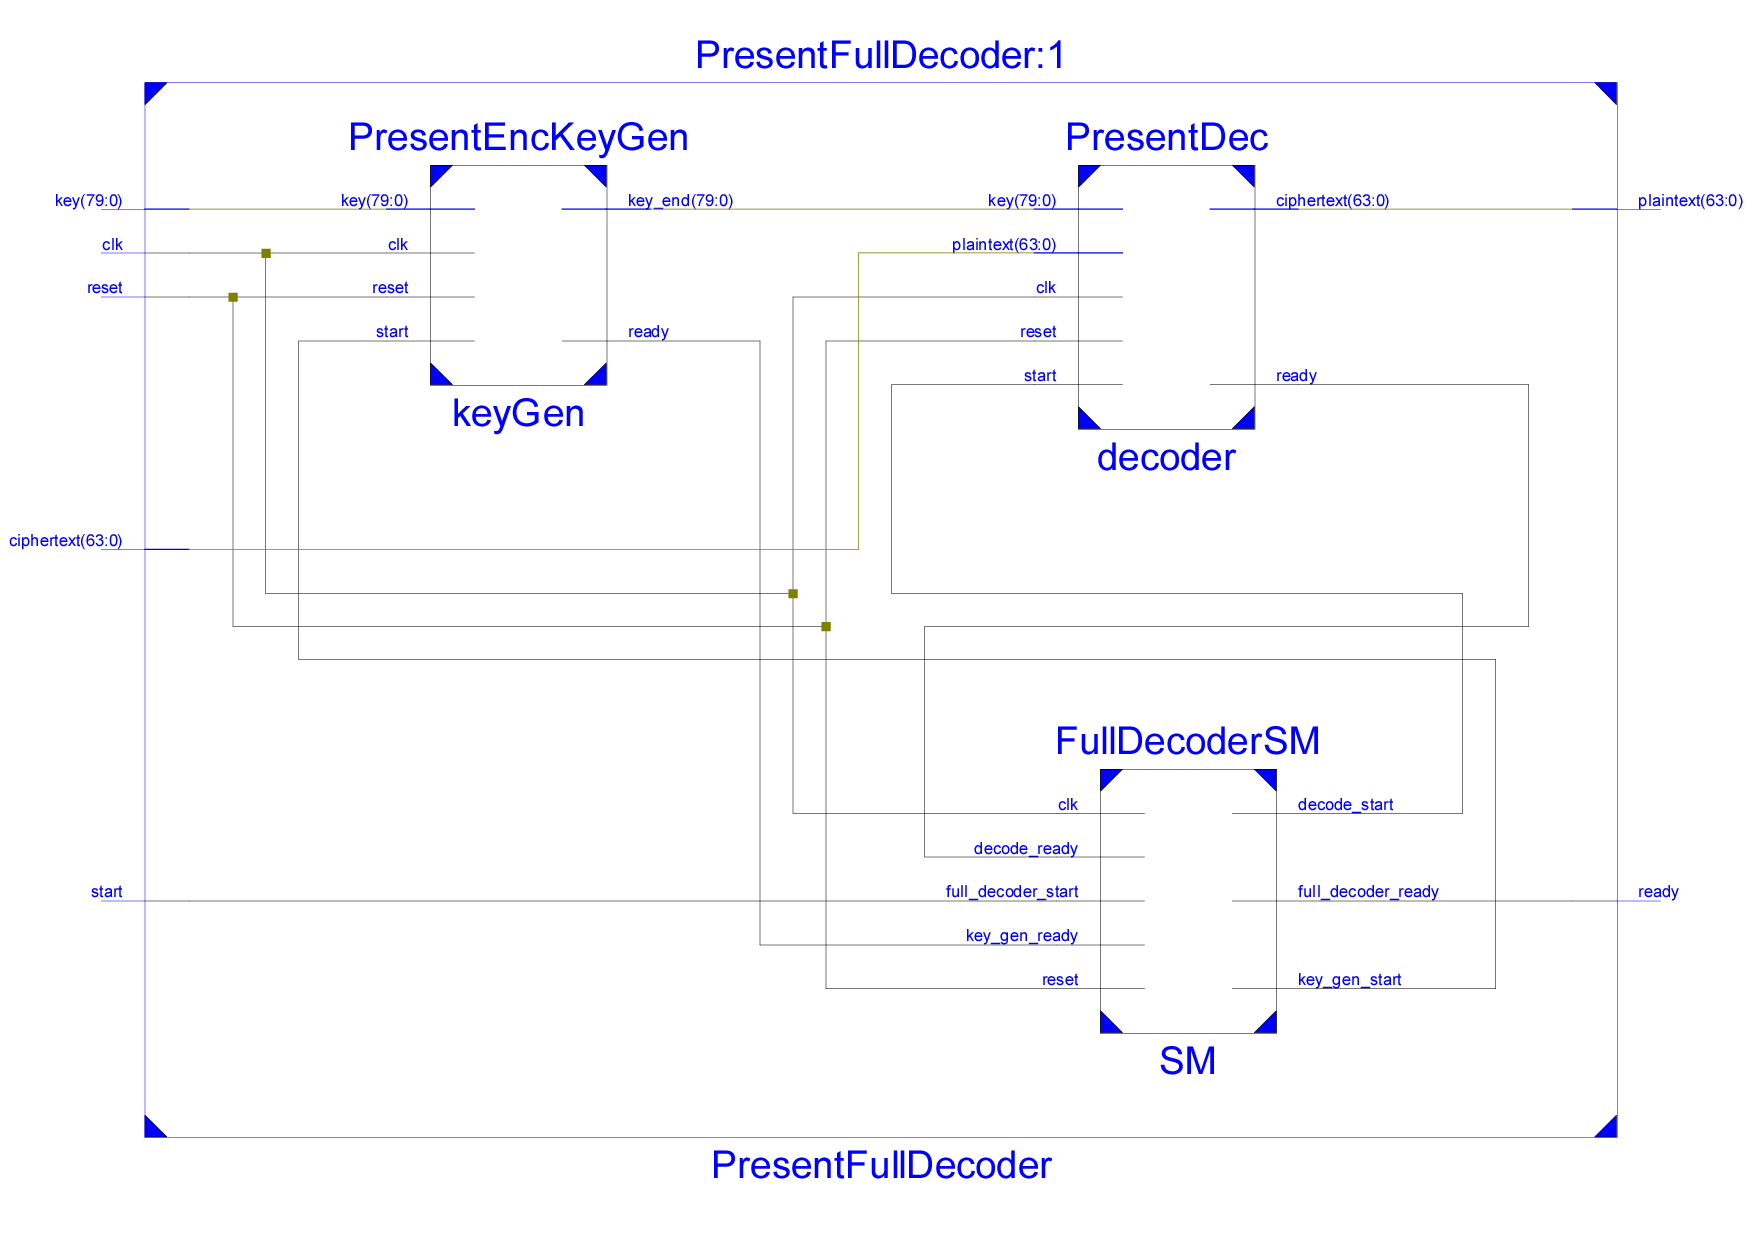
\includegraphics[width=0.8\textwidth]{img/internalStructure.png}
    \caption{%
        Internal datapath between main components in the Present decoder.
     }%
    \label{internalStructure}
    \end{center}
 \end{figure}

Internal datapath between main components was shown in Fig. \ref{internalStructure}. They are responsible for:

\begin{itemize}
    \item \texttt{PresentEncKeyGen} - key generator for decoding process. Before decoding stage, key need to be prepared to the 'appropriate value'. This value is signalled by \texttt{ready = '1'}. It is almost the same core as in \texttt{Present} subproject, but truncated from text encoding part.
    \item \texttt{PresentDec} - subcomponent responsible for ciphertext decoding. It is working in similar way as Present cipher, but is working in inverse way.
    \item \texttt{FullDecoderSM} - State machine controlling overall decoding process.
\end{itemize}

More information about cipher core and key generation process can be found in \\ \texttt{./Present/doc/present\_pure.pdf} file ("Present" subproject documentation).

\begin{figure}[!ht]%
    \begin{center}
    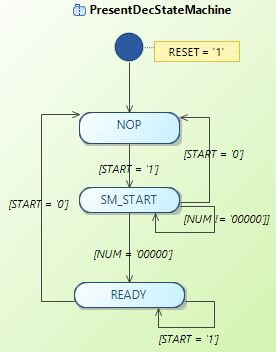
\includegraphics[width=0.4\textwidth]{img/PresentDecStateMachine.jpg}
    \caption{%
        State machine of the Present component
     }%
    \label{presentDecSM}
    \end{center}
 \end{figure}

State machine of the \texttt{PresentDec} component was shown in Fig. \ref{presentDecSM}. It consists of three states \texttt{NOP}, \texttt{SM\_START} and \texttt{READY}. The way of work of this state machine is the same as in the \texttt{Present} subproject, but the counter is counting down instead of counting up.

\begin{figure}[!ht]%
    \begin{center}
    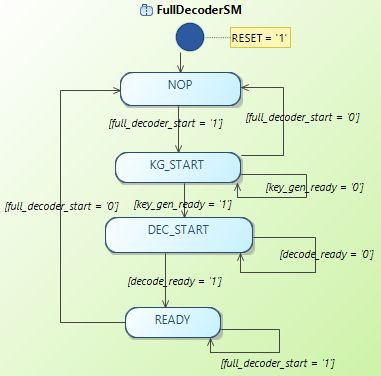
\includegraphics[width=0.5\textwidth]{img/FullDecoderSM.jpg}
    \caption{%
        State machine of the Present decoder in main component.
     }%
    \label{presentFullDecSM}
    \end{center}
 \end{figure}

State machine of the \texttt{FullDecoderSM} component was shown in Fig. \ref{presentFullDecSM}. It consists of four states \texttt{NOP}, \texttt{KG\_START}, \texttt{DEC\_START} and \texttt{READY}. \texttt{NOP} is the default state after resetting the core. This state is active as long as \texttt{full\_decoder\_start} = '0'.

When \texttt{full\_decoder\_start} = '1' key generation for the decoding process starts. Proper \texttt{key} and \texttt{ciphertext} must feed the input before. \texttt{KG\_START} state is active as long \texttt{PresentEncKeyGen} is generating the key. Key generation ends, when \texttt{PresentEncKeyGen} sets the \texttt{ready} signal to '1'. When the \texttt{ready} signal is set to '1', the state is changing.

During \texttt{DEC\_START} state decoding process appears. State machine is in this state until \texttt{PresentDec} ends its works. The end of decoding is signalled by setting the \texttt{ready} signal to '1' by the \texttt{PresentDec} component. Then, the state is changing.

\texttt{READY} state sets the \texttt{ready} signal of the \texttt{PresentFullDecoder} to '1'. It is idle-like state, when user can read the output of the Present decoder. The state machine is in this state until user sets the \texttt{full\_decoder\_start} to '0'.

\newpage

\section{FPGA implementations}

The  component  has  only  been  verified on a Xilinx\textsuperscript{\textregistered} Spartan 3E XC3S500E FPGA in FG320 package and synthesized  with  Xilinx  ISE  14.2.  Appropriate setup files was prepared with use of ISE Project Navigator, but Makefile scripts was also written. Suitable files was stored in \texttt{./Decode/syn/XC3ES500/}  directory. 
Implementation in FPGA device was done in another subproject called \texttt{DecodeTesting}.
Makefile was tested in Windows 8 with use of Cygwin for 64-bit Windows.

Synthesis results was given in Fig. \ref{SynResults}

\begin{tabularx}{\textwidth}{|p{45mm}|p{30mm}|p{30mm}|X|}
  \hline \multicolumn{4}{|c|}{Xilinx \textregistered Spartan 3E XC3S500E FPGA in FG320 package} \\
  \hline \bf{Parameter} & \bf{Used} & \bf{Available} & \bf{Utilisation}\\ 
  \hline Number of Slices & 354 & 4656 & 7\% \\
  \hline Number of Slice Flip Flops & 240 & 9312 & 2\% \\
  \hline Number of 4 input LUTs & 402 & 9312 & 4\% \\
  \hline Number of bonded IOBs & 212 & 232 & 91\% \\
  \hline Number of GCLKs & 1 & 24 & 4\%\\
  \hline Minimum period & 5.023ns & - & - \\
  \hline Maximum Frequency & 199 MHz & - & - \\
  \hline
\end{tabularx}
\label{SynResults}
\captionof{table}{Synthesis results for Spartan 3E XC3S500E}

Possible change in used FPGA device may be possible in steps given below\footnotemark[1]:
\begin{enumerate}
    \item Copy \texttt{./Decode/syn/XC3ES500/} directory to another one like \texttt{./Decode/syn/YOUR\_FPGA\_SYMBOL/}
    \item Go to \texttt{./Decode/syn/YOUR\_FPGA\_SYMBOL/}  directory.
    \item In \texttt{PresentFullDecoder.xst} file modify the line \texttt{-p xc3s500e-5-fg320} to \texttt{-p YOUR\_FPGA\_CODE}
    \item In \texttt{Makefile} file modify the line \texttt{PLATFORM=xc3s500e-fg320-5} to \texttt{PLATFORM=YOUR\_FPGA\_CODE}
\end{enumerate}

\footnotetext[1]{This solution was not tested and is based on my own observations.}


\newpage

\section{Simulation}

Self-checking test bench were provided to the components used for the Present encoder. They are stored in \texttt{./Decode/bench/vhdl} directory. Suitable configuration files and Makefile used for running test bench was stored in 
\texttt{./Decode/sim/rtl\_sim/bin} directory. Appropriate test vectors was taken from \cite{PRESENT}.

Makefile was prepared to make "manual run" of tests. If You want to perform it without gui, remove \texttt{-gui} option in Makefaile.

\newpage

\section{Troubleshooting}

During work with Windows 8 64-bit and and Xilinx\textsuperscript{\textregistered} ISE 64-bit some problems may occur:

\begin{enumerate}
    \item Xilinx may be unable to open projects in Project Navigator.
    \item When you run \texttt{make} in Cygwin and perform testbench it would be unable to open ISIM gui.
    \item When you run ISIM gui  (*.exe test bench file) it hangs out or anti virus protection opens.
\end{enumerate}

To solve problems listed above you have to perform steps listed below:
\begin{enumerate}
    \item You have to rename libraries \texttt{libPortabilityNOSH.dll} to \texttt{libPortability.dll} from \texttt{nt64} directories (\href{http://www.gadgetfactory.net/2013/09/having-problems-installing-xilinx-ise-on-windows-8-64bit-here-is-a-fix-video-included/}{http://www.gadgetfactory.net/2013/09/having-problems-installing-xilinx-ise-on-windows-8-64bit-here-is-a-fix-video-included/})
    \item Firstly, install Cygwin X11 (\href{http://stackoverflow.com/questions/9393462/cannot-launch-git-gui-using-cygwin-on-windows}{http://stackoverflow.com/questions/9393462/cannot-launch-git-gui-using-cygwin-on-windows})
    \item Temporary switch off anti virus protection.
\end{enumerate}

\newpage

\section{License and Liability}

Copyright \textcopyright  2013 Authors and OPENCORES.ORG

This source file may be used and distributed without
restriction provided that this copyright statement is not
removed from the file and that any derivative work contains
the original copyright notice and the associated disclaimer.

This source file is free software; you can redistribute it
and-or modify it under the terms of the GNU Lesser General
Public License as published by the Free Software Foundation;
either version 2.1 of the License, or (at your option) any
later version.

This source is distributed in the hope that it will be
useful, but WITHOUT ANY WARRANTY; without even the implied
warranty of MERCHANTABILITY or FITNESS FOR A PARTICULAR
PURPOSE. See the GNU Lesser General Public License for more
details.

You should have received a copy of the GNU Lesser General
Public License along with this source; if not, download it
from \href{http://www.opencores.org/lgpl.shtml}{http://www.opencores.org/lgpl.shtml}

Xilinx, Spartan3E is registered trademark of Xilinx Inc. 2100 Logic Drive, San Jose CA USA

\newpage

\bibliography{bibliography}

\end{document}
